\documentclass[11pt, a4paper]{article}
\usepackage{parskip}
%\usepackage[utf8]{inputenc} % Umlaute moussen nicht maskiert werden
\usepackage{fontspec} % Umlaute im eps sind nicht zusammengesetzt
\usepackage{lmodern} % Vektor-Schriftart
%\usepackage{ngerman} % Deutsche Silbentrennung (texlive-german und texlive-hyphen-german)
\usepackage{polyglossia}
\setmainlanguage{german}
\usepackage{graphicx} % Einbinden von Grafiken / SVG-Dateien moussen zuvor als eps exportiert werden
\usepackage{url} % Four URLs in der Bibliographie
\usepackage{amstext} % Four nichtkursiven Text in Formeln
\usepackage{listings}
\lstset{literate=%
	{Ö}{{\"O}}1
	{Ä}{{\"A}}1
	{Ü}{{\"U}}1
	{ß}{{\ss}}1
	{ü}{{\"u}}1
	{ä}{{\"a}}1
	{ö}{{\"o}}1
	{~}{{\textasciitilde}}1
}
\usepackage[dvipsnames]{xcolor}
\lstset{
	numbers= left,
	language=C++,
	keywordstyle=\color{Blue},
	stringstyle=\color{Orange},
	commentstyle=\color{OliveGreen},
	breaklines=true,
	extendedchars=true,
	basicstyle=\footnotesize\ttfamily,
	tabsize=4,
	frame=single,
	rulecolor=\color{black},
	captionpos=b,
	morekeywords={Vector3, Matrix, Transform, Vector4, Vector6,  EulerAngleXYZVector, Position, Vector, Rotation}}
\lstset{literate={-}{{-\allowbreak}}{1} }

\usepackage[export]{adjustbox}

\usepackage{etoolbox}% http://ctan.org/pkg/etoolbox
\makeatletter
\patchcmd{\lst@GLI@}% <command>
{\def\lst@firstline{#1\relax}}% <search>
{\def\lst@firstline{#1\relax}\def\lst@firstnumber{#1\relax}}% <replace>
{\typeout{listings firstnumber=firstline}}% <success>
{\typeout{listings firstnumber not set}}% <failure>
\makeatother
\newcommand{\code}{\texttt}
\usepackage{textcomp}
\usepackage{gensymb}
\usepackage{float}
\usepackage{csquotes}
\usepackage{amsmath}
\usepackage{microtype}
\usepackage{tikz}
\usepackage{xcolor}
\usetikzlibrary{shapes}
\date{\today}
\hyphenation{Trans-for-ma-ti-ons-ma-t-ri-zen, Trans-for-ma-ti-ons-ma-t-rix,Ko-or-di-na-ten-sys-teme,Ko-or-di-na-ten-sys-tem}
\begin{document}
\begin{center}
{\Huge Hochschule Darmstadt} \\
\vspace{0.5cm}
Lehrveranstaltung: Simulation von Robotersystemen \\
Dozent: Prof. Dr. Thomas Horsch \\
Laboringenieur: Rudi Scheitler \\
Versuch: Konfigurationsraum\\
Datum: 10.6.2016 \\
\vfill
\renewcommand{\arraystretch}{2}
	\begin{tabular}{| l | l |}
	\hline
	Name & Matrikelnummer \\ \hline
	Fabian Alexander Wilms & 735162 \\ \hline
	\end{tabular} \\
\vspace{0.5cm}
Studiengang: Mechatronik \\
Abgabedatum: 17.6.2016 \\
\renewcommand{\arraystretch}{1}
\end{center}
\newpage
\tableofcontents
\newpage
Ein Konfigurationsraum stellt grafisch dar, für welche Gelenkstellungen ein Roboter mit der Umgebung kollidiert. Für zwei Gelenkvariablen lässt sich dies in einem x-y-Diagramm darstellen.

Das Ziel dieses Praktikums ist es, für zwei gegebene Roboter samt Umgebungen jeweils einen Konfigurationsraum zu bestimmen. Dabei beschränken wir uns auf Modelle in der Ebene.

\section{Translatorischer Roboter}
In der ersten Aufgabe ist ein quadratischer TT-Roboter (2 translatorische Freiheitsgrade in x- und y-Richtung) gegeben. Um die Nulllage herum befinden sich 5 Rechtecke, welche die Hindernisse darstellen. Um sich dies besser vorstellen zu können und den resultierenden Konfigurationsraum einfacher auf Korrektheit überprüfen zu können, ist zudem eine EasyRob .cel-Datei gegeben, die Roboter und Umgebung enthält. In EasyRob können allerdings nur dreidimensionale Modelle hinzugefügt werden, weshalb alle Rechtecke zu Quadern extrudiert sind.

\begin{figure}[H]
\center\begin{tikzpicture}[scale = 7]
\fill[red,shift = {(-0.7, -0.4)}] (0,0) rectangle (0.3,0.05); %0
\fill[red,shift = {(-0.25, -0.3)}] (0,0) rectangle (0.05,0.6); %1
\fill[red,shift = {(-0.2, 0.45)}] (0,0) rectangle (0.25,0.05); %2
\fill[red,shift = {(-0.15, -0.25)}] (0,0) rectangle (0.55,0.05); %3
\fill[red,shift = {(-0.05, 0.2)}] (0,0) rectangle (0.1,0.05); %4
\fill[red,shift = {(0.05, 0-.6)}] (0,0) rectangle (0.05,0.2); %5
\fill[red,shift = {(0.25, 0.25)}] (0,0) rectangle (0.05,0.25); %6
\fill[red,shift = {(0.35, -0.5)}] (0,0) rectangle (0.05,0.25); %7
\fill[red,shift = {(0.45, 0.15)}] (0,0) rectangle (0.2,0.05); %8
\fill[red,shift = {(0.2, -0.15)}] (0,0) rectangle (0.05,0.3); %9
\fill[blue,shift = {(0, 0)}] (0,0) rectangle (0.07,0.07); %0
\draw[->] (-0.6,0) -- (0.6,0) node [anchor = west] {X};
\draw[->] (0,-0.6) -- (0,0.6) node [anchor = south] {Y};
\foreach \x in {-500,500} { \node [anchor=north] at (\x/1000,0) {\x}; }
\foreach \y in {-500,500} { \node [anchor=east,fill=white,inner sep=0,outer sep=0,xshift=-0.1cm] at (0,\y/1000) {\y}; }
\end{tikzpicture}
\caption{Roboter in Nullstellung (blau) und Hindernisse (rot)}
\end{figure}

Roboter und Umgebung werden in C++ mithilfe der Klasse \code{Box} aus der OPCODE-Bibliothek modelliert. Diese Bibliothek ermöglicht eine ressourcensparende Kollisionserkennung. Ein Objekt dieser Klasse hat 9 Freiheitsgrade: Skalierung, Translation und Rotation im Raum. Der Konfigurationsraum wird im zweidimensionalen Array \code{cspace} gespeichert. \code{cspace}  ist implementiert als Array  der Größe \code{height}, welches in jedem Feld ein Array der Größe \code{width} vom Typ \code{char} enthält.

Die skalierten und verschobenen Objekte vom Typ \code{Box} werden in zwei weiteren Array gespeichert: \code{aRobot} und \code{aHindernis}.

Die eigentliche Bestimmung des Konfigurationsraums findet mithilfe von vier verschachtelten \code{for}-Schleifen statt. Die äußere durchläuft alle möglichen Werte für Gelenkvariable 1 von 0 bis \code{width}. Die nächste Schleife durchläuft alle möglichen Werte für Gelenkvariable 2 von 0 bis \code{height}. Damit steht innerhalb dieser zweiten Schleife die Position des Roboters fest. Mittels der Methode \code{Box::Translate()} wird der Roboter an diese Stelle unter Beachtung des Offsets von -500 in beide Richtungen verschoben. Die nächsten beiden Schleifen durchlaufen alle Hindernis- und Armteilindizes. Innerhalb dieser wird mithilfe der Funktion \code{collide()} abgefragt, ob für die gegebenen Gelenkwinkel das Hindernis \code{k} mit dem Armteil \code{l} kollidiert. Ist das der Fall, so wird das Feld \code{cspace[height - 1 - j][i]} um den um 1 inkrementierten Hindernisindex inkrementiert. Auf diese Art auf die Felder von \code{cspace} zuzugreifen ist nötig, da zwar \code{i} im Array und X im Modell in dieselbe Richtung zeigen, \code{j} und Y jedoch in entgegengesetzte.
\vspace{11pt}
\lstinputlisting[firstline=84,lastline=116,caption={Bestimmung des Konfigurationsraums}]{../Termin5/PrismaticJoints/main.cpp}

Die Ausgabe des Programms lautet wie folgt:

\begin{lstlisting}
Berechnung dauerte 14586 ms
Anzahl Kollisionstests: 10000000
Anzahl Kollisionen: 2146190
Anteil Kollisionen: 0.214619
PNG erfolgreich erzeugt
\end{lstlisting}

Basierend auf den Werten, die nun in der Variablen \code{cspace} stehen wird diese Visualisierung des Konfigurationsraums erstellt:

\begin{figure}[H]
\center\begin{tikzpicture}
\node[anchor=south west,inner sep=0] (image) at (0,0)	{
\includegraphics[width=0.5\textwidth]{cspace_prismatic.png}};
\begin{scope}[x={(image.south east)},y={(image.north west)}]
\draw[->] (-0.1,0.5) -- (1.1,0.5) node [anchor = west] {X};
\draw[->] (0.5,-0.1) -- (0.5,1.1) node [anchor = south] {Y};
%\draw[help lines,xstep=.1,ystep=.1] (0,0) grid (1,1);
\foreach \x in {-500,500} { \node [anchor=north] at (\x/1000+0.5,0.5) {\x}; }
\foreach \y in {-500,500} { \node [anchor=east,fill=white,inner sep=0,outer sep=0,xshift=-0.1cm] at (0.5,\y/1000+0.5) {\y}; }
\end{scope}
\end{tikzpicture}
	\caption{Konfigurationsraum des TT-Roboters}
\end{figure}

Es ist erkennbar, dass man die Minkowski-Summen der des Roboters und der jeweiligen Hindernisse gebildet hat, wodurch die Hindernisse im Konfigurationsraum größer erscheinen. Das heißt, dass man mit der Koordinate, die die Position des Roboters auszeichnet nicht beliebig nah an die Hindernisse heranfahren kann, da der Roboter auch eine Ausdehnung hat.

\section{Rotatorischer Roboter}

Dieselbe Methode zur Bestimmung des Konfigurationsraumes soll nun auf einen RR-Roboter (2 rotatorische Freiheitsgrade, Rotationsachse z) angewandt werden.

Es werden wieder vier verschachtelte Schleifen verwendet, nur die Art, auf die die Armteile transformiert werden, unterscheidet sich zum TT-Roboter. Die zwei äußeren Schleifen durchlaufen mit den beiden Gelenkvariablen jeweils Werte von 0° bis 360°. Diese Werte werden, um den Offset von -180° bereinigt in dem zweidimensionalen Vektor \code{axes} gespeichert. Mit der Funktion \code{ForwardKinematics()} werden dann die Transformationsmatrizen der beiden Armteile bestimmt. Mit diesen sollen die als \code{Box} modellierten Armteile transformiert werden. Da diese Funktion auf der Vectmath-Bibliothek aufbaut, \code{Box} aber auf der OPCODE-Bibliothek, sind die Transformationsmatrizen nicht gleich aufgebaut. Daher müssen die auf die \code{Box}-Objekte anzuwendenden Transformationsmatrizen manuell aus den mittels der Vorwärtskinematik berechneten Matrizen zusammengestellt werden.
\begin{figure}[H]
	\center\begin{tikzpicture}[scale = 8]
	\fill[blue,shift = {(0.2, 0.15)}] (0,0) rectangle (0.1,0.1); %0
	\fill[blue,shift = {(0, 0.25)}] (0,0) rectangle (0.04,0.1); %1
	\fill[blue,shift = {(0.25, -0.15)}] (0,0) rectangle (0.04,0.1); %2
	\fill[blue,shift = {(-0.25, -0.15)}] (0,0) rectangle (0.2,0.05); %3
	\fill[blue,shift = {(-0.3, 0.1)}] (0,0) rectangle (0.1,0.2); %4
	\fill[lightgray,shift = {(0, 0)}] (0,0) rectangle (0.18,0.05); %0
	\fill[gray,shift = {(0.18, 0)}] (0,0) rectangle (0.23,0.05); %0
	\draw[->] (-0.6,0) -- (0.6,0) node [anchor = west] {X};
	\draw[->] (0,-0.6) -- (0,0.6) node [anchor = south] {Y};
	\foreach \x in {-500,500} { \node [anchor=north] at (\x/1000,0) {\x}; }
	\foreach \y in {-500,500} { \node [anchor=east,fill=white,inner sep=0,outer sep=0,xshift=-0.1cm] at (0,\y/1000) {\y}; }
	\end{tikzpicture}
	\caption{Roboter in Nullstellung (grau) und Hindernisse (blau)}
\end{figure}

\lstinputlisting[firstline=97,lastline=154,caption={Bestimmung des Konfigurationsraumes}]{../Termin5/RevoluteJoints/main.cpp}

Die Ausgabe des Programms lautet wie folgt:

\begin{lstlisting}
Berechnung dauerte 3261 ms
Anzahl Kollisionstests: 1296000
Anzahl Kollisionen: 264661
Anteil Kollisionen: 0.204214
PNG erfolgreich erzeugt
\end{lstlisting}
\newpage
Es ergibt sich folgender Konfigurationsraum: 

\begin{figure}[H]
	\center\begin{tikzpicture}
	\node[anchor=south west,inner sep=0] (image) at (0,0)	{
\includegraphics[width=0.5\textwidth]{cspace_revolute.png}};
	\begin{scope}[x={(image.south east)},y={(image.north west)}]
	\draw[->] (-0.1,0.5) -- (1.1,0.5) node [anchor = west] {q\textsubscript{1}};
	\draw[->] (0.5,-0.1) -- (0.5,1.1) node [anchor = south] {q\textsubscript{2}};
	\foreach \x in {-180,180} { \node [anchor=north,fill=white,inner sep=0,outer sep=0,yshift=-0.1cm] at (\x/360+0.5,0.5) {\x°}; }
	\foreach \y in {-180,180} { \node [anchor=east,fill=white,inner sep=0,outer sep=0,xshift=-0.1cm] at (0.5,\y/360+0.5) {\y°}; }
	\end{scope}
	\end{tikzpicture}
	\caption{Konfigurationsraum des RR-Roboters}
\end{figure}

Es ist erkennbar, dass die Werte bei +180° und -180° in beiden Richtungen übereinstimmen, da die Armteile in diesen Fällen jeweils dieselbe Position und Rotation haben. Damit sind auch die Kollisionen dieselben.

Zwischen Werten von -164° bis -108° für $q_1$ ist ein für alle Werte von $q_2$ durchgehendes Band zu erkennen. Die bedeutet, dass für diese Gelenkstellungen eine Kollision von Armteil 1 unvermeidbar ist. Ähnliches gilt für Armteil 2. Dies lässt sich mit EasyRob leicht verifizieren:

\begin{figure}[H]
	\centering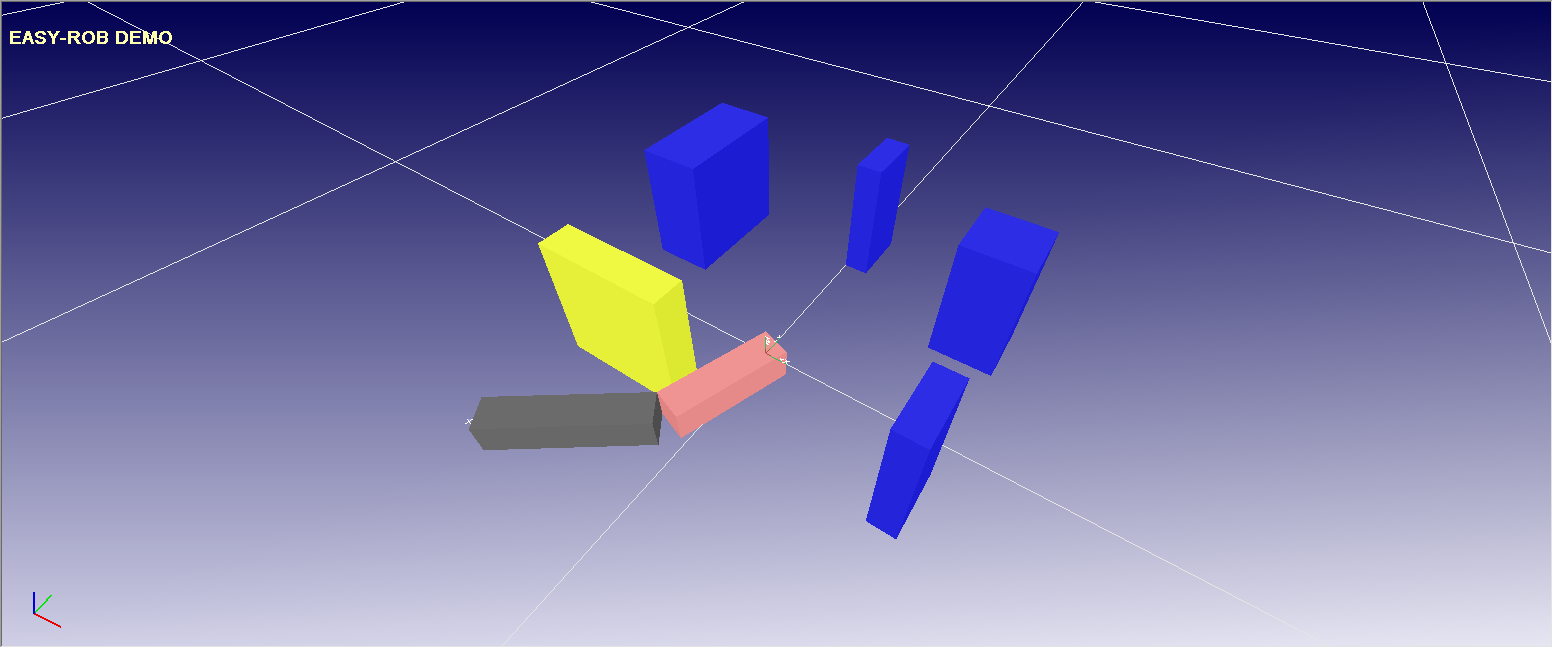
\includegraphics[width=0.7\textwidth]{revolute-easyrob.png}
	\caption{Kollision von Armteil 1}
\end{figure}

\end{document}